\documentclass[10pt,twocolumn,letterpaper]{article}

\usepackage{cvpr}
\usepackage{times}
\usepackage{epsfig}
\usepackage{graphicx}
\usepackage{amsmath}
\usepackage{amssymb}
\usepackage{multirow}
\usepackage{subfigure}
\usepackage[colorlinks,linkcolor=black,anchorcolor=blue,citecolor=green, urlcolor = blue, breaklinks=true,bookmarks=false]{hyperref} % Using hyper reference
\usepackage{indentfirst}

\cvprfinalcopy

\def\httilde{\mbox{\tt\raisebox{-.5ex}{\symbol{126}}}}

\begin{document}
\title{
  Report of SJTU MVIG Training Section II
}
\author{
  Zelin Ye\\
  Shanghai Jiao Tong University\\
  \tt \small \  542782758@qq.com
}
\maketitle

\begin{abstract}
	Recently, Deep Reinforcement Learning (DRL) has becoming more and more popular. During this period of time, I have also learned some related knowledges and implemented some algorithms referring to some great projects and papers like \cite{DQN_nature,Double_DQN,Dueling_network}.
	
	In this report, I not only introduce some basic theories of Reinforcement Learning according to \cite{DQN_zhihu,RL_zhihu,DQN_csdn}(Because it can be regarded as the foundation of DRL in some way, some algorithms are based on it), but also illustrate three classic DRL algorithms, DQN, Double DQN and Dueling network.
	
	To the three algorithms, except for introducing their basic theories and architecture, I also show some implement details of them.
	
	At the end of this report, I conclude testing results and analysis of three models. Then I summarize this training stage, both in knowledges and practices. Ultimately, I express my wishes to the future.
\end{abstract}

\section{Introduction}

After half a month studying on Deep Reinforcement Learning(DRL), I have gone through many related materials, papers, codes and projects, which do help me master the basic concepts, theories and some classical algorithms of DRL.

In addition to learning theoretical knowledges, I also put these theories into practice. In the beginning, I implement the Deep Q-learning algorithm(DQN) referring to \cite{github_code1,github_code2}(Basically, I use most of their codes) and apply it to an Atari game called \textit{breakout}. However, there exist some drawbacks in DQN algorithm, like overestimations. Therefore, I use Double DQN algorithm and Dueling network to improve or replace the original DQN algorithm. I train models in \textit{breakout} game with three different algorithms, and some differences do appear, which are a little bit different from what I have imagined. After that, I try to change the architecture of DQN network to find something different.

The following sections are about some basic concepts of Reinforcement Learning(RL), the three algorithms, some details of my implementations and corresponding experiment results.

In this paper, I will try my best to use my own words to introduce the basic concepts instead of just copying related papers, there may be some inaccuracies or even errors in my statements, please just point them out and let me know in time.

\section{Basic Theories}
	\subsection{Reinforcement Learning}
	Fundamentally, RL can be considered as a kind of algorithm. What problem RL tries to solve is how an agent can finish a certain task greatly just by interacting with environment. 
	
	In this process, there are some vital concepts: action, state and reward. These concepts will be discussed later. In short, the process of RL can be described like this: 
	
	An agent takes an action, then it comes to a new state, may be better or worse. In the meantime, it will receive a reward. According to this reward, the agent will adjust its policy to approach the best one. 
	
	The so-called policy, is a mapping from states to actions, that is, the agent in a state \textbf{\textit{s}} will use its policy to decide a certain action \textbf{\textit{a}}. Therefore, in mathematics, the policy can be described as
	
	\begin{center}
		$a=\pi(s)$
	\end{center}
	
	Such kind of algorithm is called Reinforcement Learning (RL).
	
	\subsection{Markov Decision Process}
	Markov Decision Process(MDP) is the foundation of RL, we can transfer RL into a MDP model. However, MDP has its own condition. A state \textit{\textbf{$s_{t}$}} can be considered as Markov iff the next state depends only on the current state and action.
	
	To describe the concept in a mathematical way, there have a simple equation (\textit{P} represents probability):
	
	\begin{center}
		$P$
		(\textit{\textbf{$s_{t+1}$}}$|$\textit{\textbf{$s_{t}$}})
		$=$
		$P$
		(\textit{\textbf{$s_{t+1}$}}$|$\textit{\textbf{$s_{t}$}},
		\textbf{\textit{$s_{t-1}$}},...,
		\textbf{\textit{$s_{1}$}},
		\textbf{\textit{$s_{0}$}})
	\end{center}
	
	As is illustrated before, RL can be considered as a MDP model. A MDP can be represented as a tuple (\textit{S},\textit{A},\textit{P}), namely states, actions and state transition probability (the probability that the agent comes to state \textbf{\textit{$s_{t+1}$}} according to current state \textbf{\textit{$s_{t}$}} and action \textbf{\textit{$a_{t}$}}). If we have \textit{P}, we can calculate future state.
	
	Besides, we also need a value to describe a state, checking whether the state is good or not. The value of state st can be defined as \textbf{\textit{Return}}:
	
	\begin{center}
		\textbf{\textit{$G_{t}$}}=
		\textbf{\textit{$R_{t+1}$}}+
		$\lambda$
		\textbf{\textit{$R_{t+2}$}}+$...$=
		$\sum\limits_{k=1}^{\infty}$
		$\lambda^{k}$
		\textbf{\textit{$R_{t+k+1}$}}
	\end{center}
	
	\textbf{\textit{R}} is reward, $\lambda$ is discount factor, which means the recent feedbacks are more important, while the old feedbacks are less important.
	
	Neveras, we can not calculate \textbf{\textit{Return}} unless the process ends. So we use a value function $v(s)$ to represent potential value of a state. Value function can be considered as the expectation of rewards:
	
	\begin{center}
		$v(s)=$
		$\mathbb{E}$
		$[$
		\textbf{\textit{$G_{t}$}}
		$|$
		\textbf{\textit{$S_{t}$}}
		$=s]$
	\end{center}
	
	More details about value function can refer to the next section.
	
	\subsection{Value Function}
	Since we have defined value function, the next step is to calculate it.
	
	We merge the equations of value function and \textbf{\textit{Return}}, then we can get a new equation, called \textbf{Bellman Equation}:
	
	\begin{center}
		$v(s)=$
		$\mathbb{E}$
		$[$
		\textbf{\textit{$R_{t+1}$}}
		$+\lambda$
		$v($
		\textbf{\textit{$S_{t+1}$}}
		$)|$
		\textbf{\textit{$S_{t}$}}
		$=s]$
	\end{center}
	
	From the above eqation, we should notice that the value of current state is related to the value of next state and reward. Therefore, value function can be calculated by iteration.
	
	\subsubsection{Action-Value Function}
	The above value function represents the value of a certain state, however, there are many optional actions in each state.
	
	We need a value to discribe a state and a action, not just discribe a state, because we care both state and action. So we define Aciton-Value function
	
	\begin{center}
		$Q^{\pi}(s,a)$.
	\end{center}
	
	$\pi$ represents the Action-Value is under the policy $\pi$.\\
	
	We also use rewards to measure Action-Value. But the rewards here are the ones received after an action, while the former rewards are expection value. With these definitions, we can derive its expression:
	
	\begin{center}
		$Q^{\pi}(s,a)=$
		$\mathbb{E}$
		$_{s^{'}}$
		$[r+\lambda$
		$Q^{\pi}(s^{'},a^{'})$
		$|s,a]$
	\end{center}
	
	In practice, we will widely use Action-Value function instead of value function.
	
	\subsubsection{Optimal Value Function}
	The goal of RL is to find the best policy, which can be transferred to find optimal value function.
	
	After defining value function, with the equation in the previous section 2.3.1, we can derive the following equation:
	
	\begin{center}
		$Q^{*}(s,a)=$
		$\mathbb{E}$
		$_{s^{'}}$
		$[r+\lambda$
		$\max\limits_{a_{'}}$
		$Q^{*}(s^{'},a^{'})$
		$|s,a]$
	\end{center}
	
	There are two basic algorithms to solve \textbf{Bellman Equation}, policy iteration and value iteration, here I focus on value iteration, for it may be more important to the following content.
	
	\subsubsection{Policy Iteration}
	Policy iteration is a way to make policy converge to the optimal one. We can use \textbf{Bellman Equation} to derive policy iteration equation:
	
	\begin{center}
		$v_{k+1}(s)=$
		$\sum\limits_{a}^{}$
		$\pi$
		$(a|s)$
		$\sum\limits_{s^{'},r}$
		$p(s^{'},r|s,a)[r+\gamma$
		$v_{k}(s^{'})]$
	\end{center}
	
	Generally speaking, policy iteration has two steps. One is called \textbf{Policy Evaluation}, used to update value function. Another is \textbf{Policy Improvement}, which will generate new samples for policy evaluation by greedy policy. The relation between the two steps can refer to figure 1.
	
	\begin{figure}[!htb]
    	\centering
    	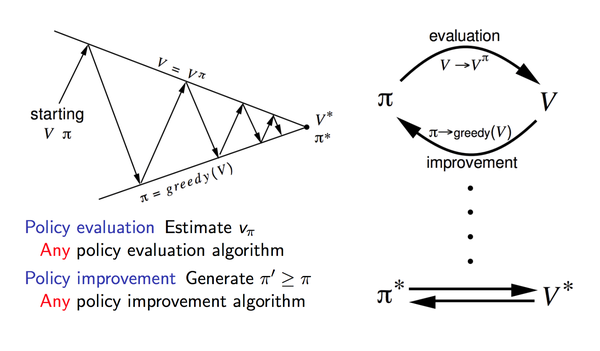
\includegraphics[width = \linewidth]{images/policy_iteration2}
    	\caption{The Relationship Between Two Steps of Policy Iteration}
    	\label{fig::policy_iteration2}
   \end{figure}
	
	In short, the whole process is using current policy to generate new samples, which will be used to evaluate the values of this policy, then the policy will be updated by such values. Repeating this process, and finally it can converge to optimal policy.
	
	For more details, please refer to its algorithm:
	
	\begin{figure}[!htb]
    	\centering
    	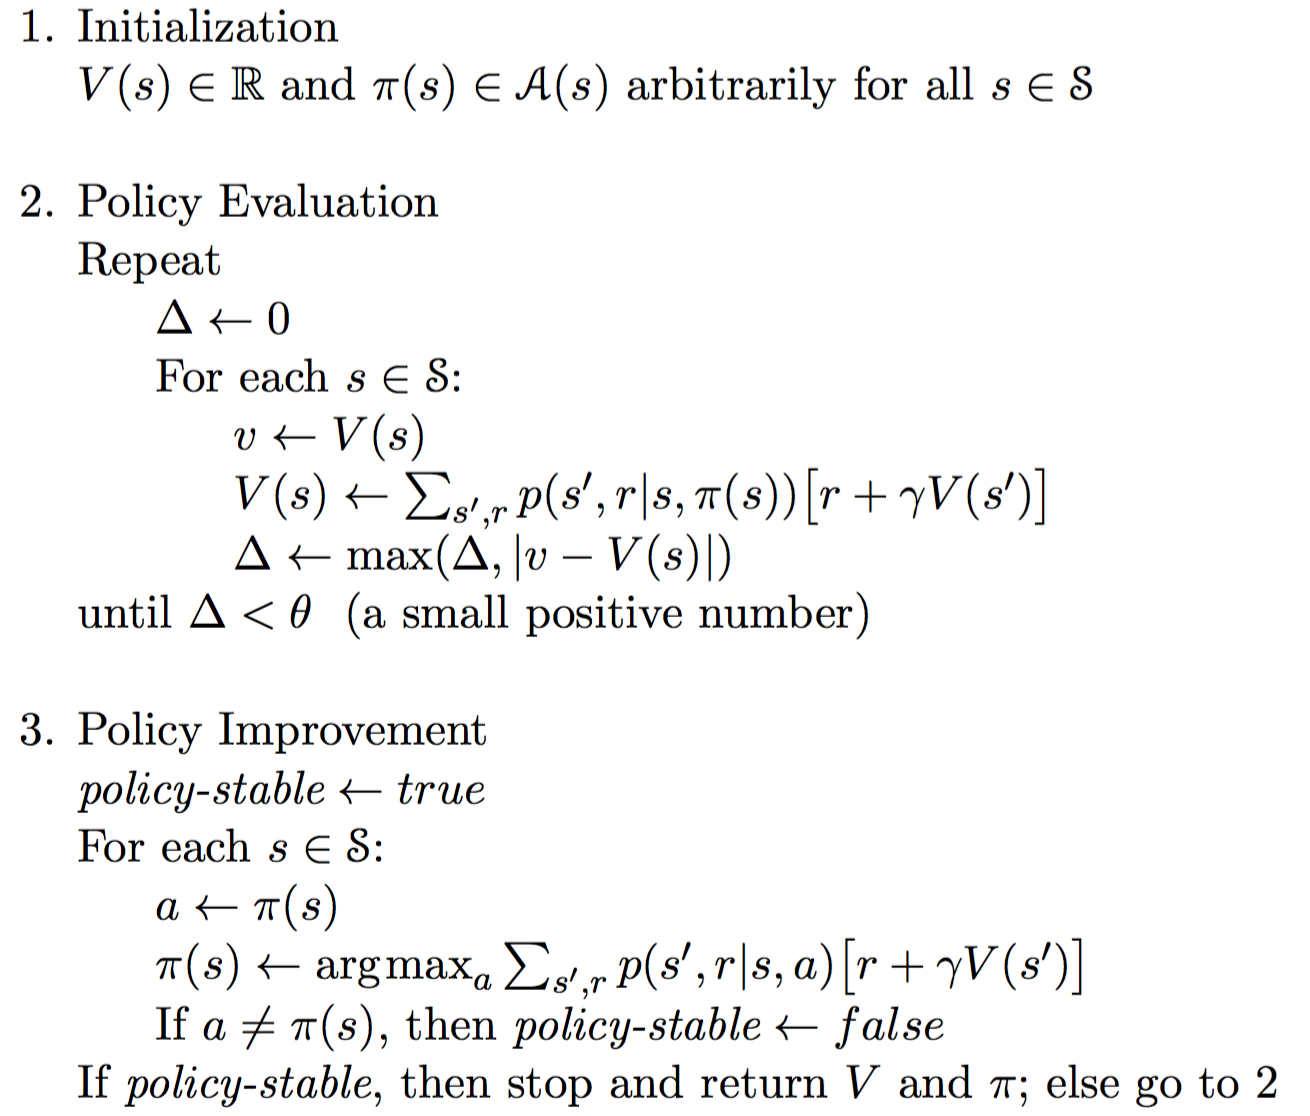
\includegraphics[width = \linewidth]{images/policy_iteration}
    	\caption{The Algorithm of Policy Iteration}
    	\label{fig::policy_iteration}
   \end{figure}
   
   Typically, the $\theta$ is the end point of this algorithm, because we can not do infinite iteration, so we define a signal $\theta$ to represent the end of iteration.
	
	\subsubsection{Value Iteration}
	We can change the original value function into the iteration type:
	
	\begin{center}
		$v_{k+1}(s)=$
		$\max\limits_{a}$
		$\sum\limits_{s^{'},r}^{}$
		$p(s^{'},r|s,a)[r+\gamma$
		$v_{k}(s^{'})]$
	\end{center}
	
	The value iteration algorithm is as follow:
	
	\begin{figure}[!htb]
    	\centering
    	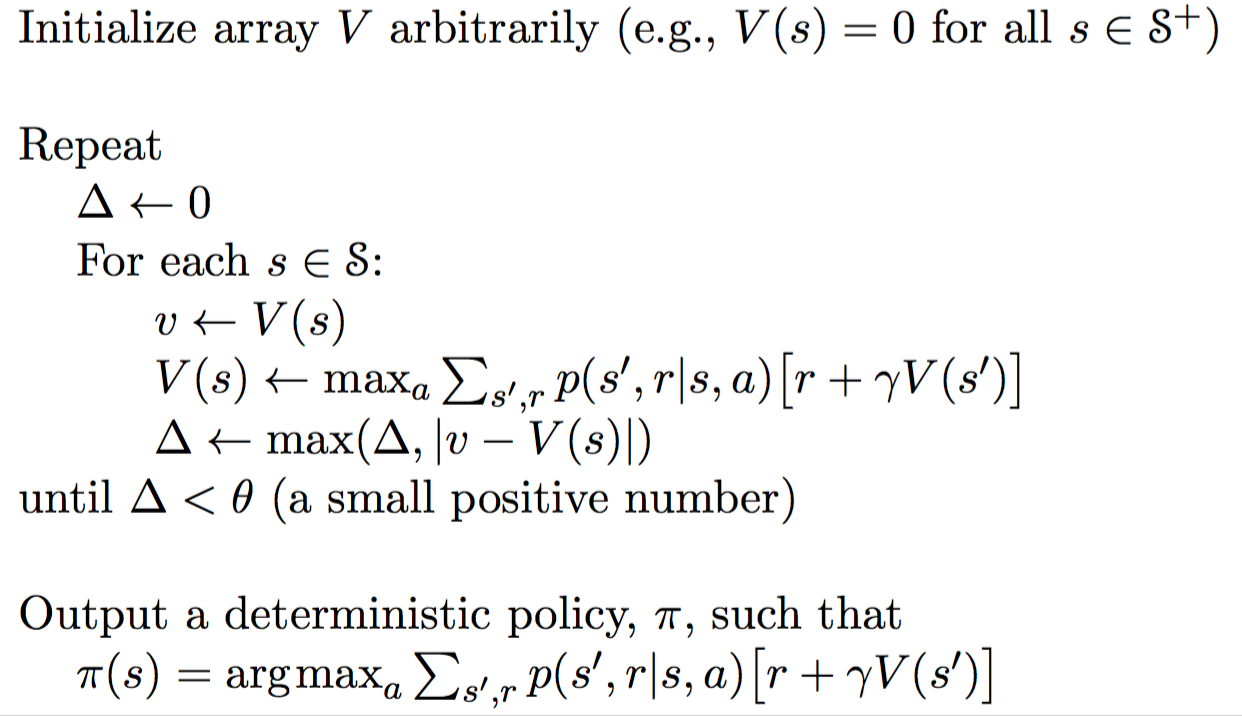
\includegraphics[width = \linewidth]{images/value_iteration}
    	\caption{The Algorithm of Value Iteration}
    	\label{fig::value_iteration}
   \end{figure}
   
   This algorithm is very straight-forward, but it depends on state transition function \textbf{\textit{p}}. Besides, in this form, it needs to ergodic all states, which is inefficient. Therefore, we generally use Action-Value function in practice, the corresponding equation is similar to its definition.
   
 	\begin{center}
 		$Q_{i+1}(s,a)=$
 		$\mathbb{E}$
 		$_{s^{'}}$
 		$[r+\lambda$
 		$\max\limits_{a_{'}}$
 		$Q_{i}(s^{'},a^{'})$
 		$|s,a]$
 	\end{center}
	
	\subsection{Q-Learning}
	The core idea of Q-Learning is from value iteration. However, different from value iteration, Q-Learning only use limited samples. Because actually, we can not ergodic all states and actions. In this case, Q-Learning has its own way to update Q value:
	
	\begin{center}
		$Q(S_{t},A_{t})\leftarrow$
		$Q(S_{t},A_{t})+\alpha$
		$(R_{t+1}+\lambda$
		$\max\limits_{a}$
		$Q(S_{t+1},a)-Q(S_{t},A_{t}))$
	\end{center}
	
	Q-Learning approaches the target Q by using a way like gradient descent. The step length depends on $\alpha$, if we choice a proper $\alpha$ value, we can greatly reduce the impact from error. We can prove this way can make Q converge to the optimal value.
	
	The detailed algorithm is as follow (I think this Chinese version makes sense and is easier to understand than some English versions, at least for me):
	
	\begin{figure}[!htb]
    	\centering
    	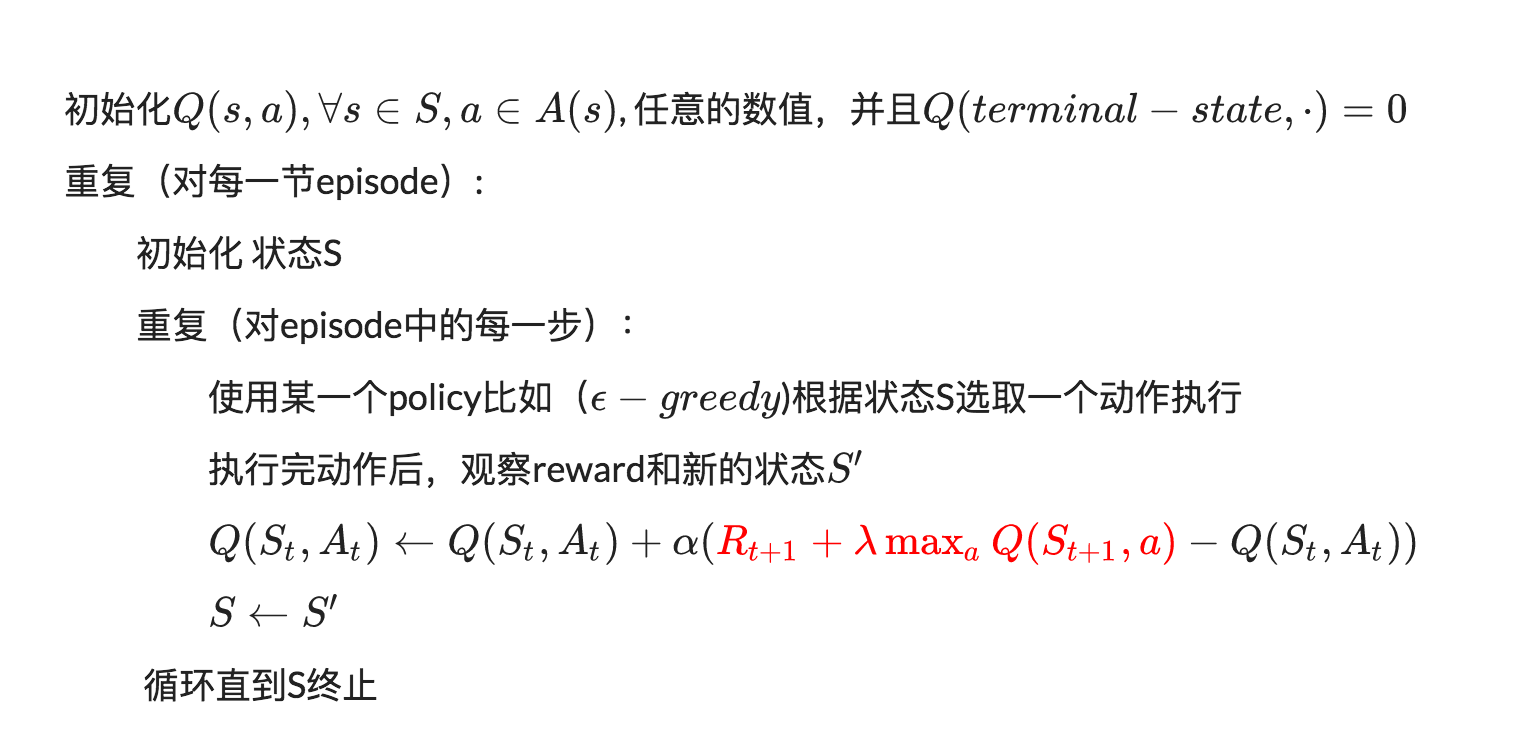
\includegraphics[width = \linewidth]{images/Q_Learning}
    	\caption{The Algorithm of Q-Learning}
    	\label{fig::Q_Learning}
   \end{figure}

\section{Network Architecture}
  \subsection{Deep Q-learning(DQN)}
   Compared with some Deep Learning network, the network of DQN is simple. In original DQN, we use 4 consecutive 84*84 images as input, and then we have 2 convolution layers and 2 full-connected layers.
   
   After these input images go through the original DQN network, we will receive a vector, which contains Q-values of actions.
   
   DQN network is a typical convolution neural network structure. And we do not use pooling layers in this network, because they will decrease the network's sensibility to the location of objects in the images. Such feature may be useful in Deep Learning field, but the location information is vital to DRL. Therefore, this network give up pooling layers.
   
   To get more details of DQN network architecture, please refer to the following figure 5 and 6.
   
   \begin{figure}[!htb]
    	\centering
    	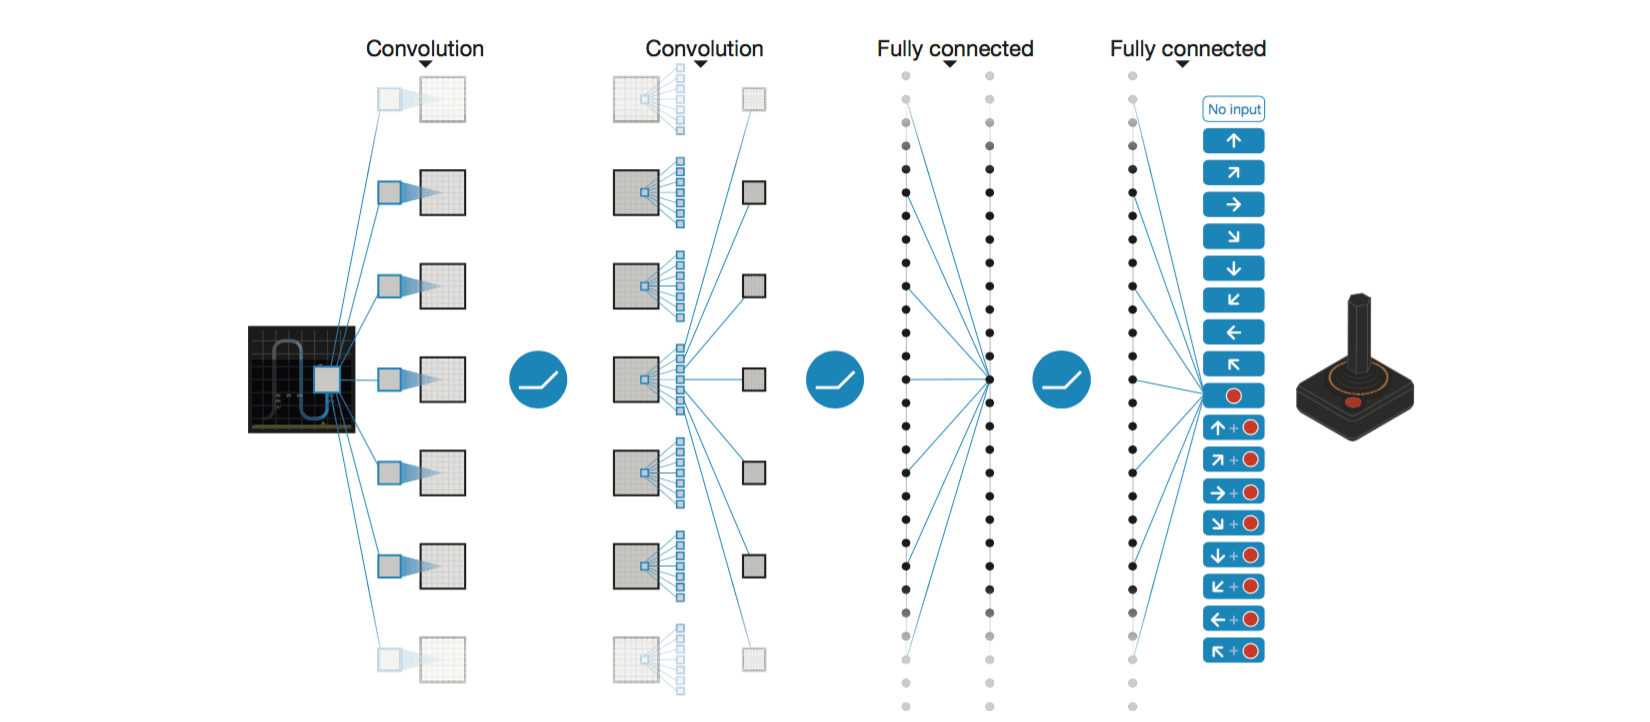
\includegraphics[width = \linewidth]{images/DQN1}
    	\caption{The Network Architecture of DQN Algorithm}
    	\label{fig::DQN1}
   \end{figure}
   
	\begin{figure}[!htb]
    	\centering
    	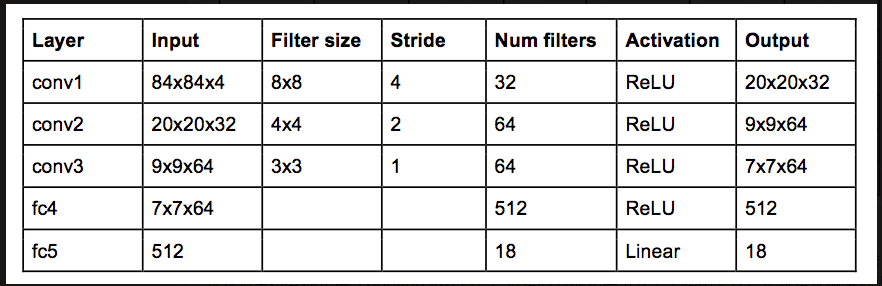
\includegraphics[width = \linewidth]{images/DQN2}
    	\caption{The Detailed Network Architecture of DQN Algorithm}
    	\label{fig::DQN2}
   \end{figure}
  
  \subsection{Double DQN}
  
    Although the DQN may work in some DRL projects, it is also known for some drawbacks, especially overestimations. The Double Q-learning algorithm(Double DQN) can solve this problem to a certain extent.
    
    Basically, there are no big changes in network architecture between DQN and Double DQN. They just use different data processing methods.
    DQN uses same values to select and evaluate an action, which is the primary cause of overestimations. In Double DQN, two value functions are learned by assigning each experience randomly to update one of the two value functions, such that there are two sets of weights, $\theta$ and $\theta^{'}$. Then the corresponding formulas in DQN should be rewritten as\\
    
    $Y^{Q}_{t}=R_{t+1}+\gamma$$Q($$S_{t+1}$,$\mathop{argmax}\limits_{a}$ $Q(S_{t+1},a;$ $\theta_{t}$)$; $$\theta_{t}$)
    
    $Y^{DoubleQ}_{t}=R_{t+1}+\gamma$$Q($$S_{t+1}$,$\mathop{argmax}\limits_{a}$ $Q(S_{t+1},a;$ $\theta_{t}$)$; $$\theta_{t}^{'}$)
    
    \subsection{Dueling Network}
    
    The Dueling network architecture can refer to figure 7.
    
	\begin{figure}[!htb]
    	\centering
    	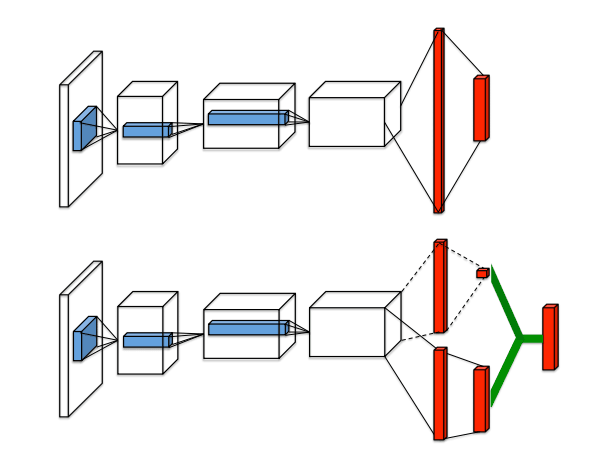
\includegraphics[width = \linewidth]{images/Dueling1}
    	\caption{The Dueling Network Architecture}
    	\label{fig::Dueling1}
   \end{figure}
    
    The top network in the figure is a popular single stream Q-network, and the Dueling Q-network is the buttom one. The Dueling network has two streams to separately estimate (scalar) state-value and the advantages for each action; the green output module implements equation ??? to combine them. Both networks output Q-values for each action.
    
    The key insight behind Dueling network architecture, is that for many states, it is unnecessary to estimate the value of each action choice. In some states, it is of paramount importance to know which action to take, but in many other states, the choice of action has no repercussion on what happens.
    
    The lower layers of the dueling network are convolutional as in the original DQNs (refer to ). However, instead of following the convolutional layers with a single sequence of fully connected layers, Dueling network uses two sequences (or streams) of fully connected layers. The streams are constructed such that they have the capability of providing separate estimates of the value and advantage functions. Finally, the two streams are combined to produce a single output Q function. As in (DQN paper), the output of the network is a set of Q values, one for each action.
    
\section{Data Processing}
	
	Different from Deep Learning, DRL does not require a large number of fixed datasets, we just need to capture the game screen and use it as raw input. Hence, I use some interfaces to get game screen, extract states information and input them into network.
	
    \subsection{The Arcade Learning Environment(ALE)}
   	ALE is a simple object-oriented framework that allows researchers and hobbyists to develop AI agents for Atari 2600 games. It is built on top of the Atari 2600 emulator Stella and separates the details of emulation from agent design.
   	
   	ALE provides the Python interface, so I can import it in my python programs and use ALE as a lib.
   	
   	With this interface, I can easily get valid actions, start a new game, check whether current game is over, and even show the game in my screen with \textbf{cv} lib.
   	
   	Indeed, although there are some other interfaces, which may do better than ALE, like OpenAI Gym. I think ALE is specialized in Atari 2600, in Atari games, ALE has its own advantages.
    
    \subsection{OpenAI Gym}
    OpenAI Gym is a toolkit for developing and comparing reinforcement learning algorithms. It supports teaching agents everything from walking to playing games like Pong or Go.
    
    It makes no assumptions about the structure of our agent, and is compatible with any numerical computation library, such as tensorFlow or Theano. It provides the Python interface, we can use it from Python code, which can be connected with famous frameworks like tensorflow.
    
    The core Gym interface is Env, which is the unified environment interface. There is no interface for agents, that part is left to programmers. The following are some of the Env methods used frequently:
    
	\begin{itemize}
 		\item \textbf{reset(self)}:Reset the environment's state. Returns observation.
 		\item \textbf{step(self, action)}: Step the environment by one timestep. Returns observation, reward, done, info.
 		\item \textbf{render(self, mode='human', close=False)}: Render one frame of the environment. The default mode will do something human friendly, such as pop up a window. Passing the close flag signals the renderer to close any such windows.
 	\end{itemize}
    
    Basically, after installing Gym, I just need to write \textit{import gym} in my Python programs, then I can make full use of the interfaces in Gym.
    
    Besides, such interface can help me construct my model without taking concrete game into consideration. That is to say, my model can be easily applied to any game supported by Gym.
    
    \subsection{Relevant Data}

    Fundamentally speaking, there are two basic concepts in DRL: the environment (namely, the outside world) and the agent (namely, the algorithm we are using). The agent sends actions to the environment, and the environment replies with states and rewards (that is, a score or some other things like that).
    
    The information we can directly get from the game are just screen images and score (if the game have it). However, we can extract following elements from the original information, which can be used in our network, either with my own codes or some interfaces like Gym or ALE.
    
	 \begin{itemize}
 		\item \textbf{States}: For \textit{breakout} game, the states would be the whole game screen consisting of many pixel points. With the help of specific interface like Gym and \textbf{cv}, I can easily get states and transfer it into a proper format, which can be received by corresponding network.
 		\item \textbf{Actions}: We can use corresponding interfaces to get all valid actions of a game, such as moving forward, turning left and etc, then store them in a matrix or some other data structures. Then the agent will select actions from these storages.
 		\item \textbf{Rewards}: After the agent taking a certain action, such action will contribute to a certain result (get one more point, lose one life or make game over). According to some mapping relations, we can transfer those results into rewards.
 	\end{itemize}
    
    Indeed, we can use integers or float numbers to represent rewards.
    
\section{Experiments}
	\subsection{Trained Models}
		
		During this period of time, I have trained three models with DQN, Double DQN and Dueling network. To Double DQN and Dueling network models, I train them about 5 millions episodes (Before announcing the report is delayed, I just train them 1 million episodes). As for DQN model, I have trained it for several days, and up to 5 millions episodes. The corresponding test results of these models can refer to table2.

	\subsection{Basical Stages}
		Based on convention, I divide the whole training process into three stages: observe, explore and train.
	
		\begin{itemize}
			\item \textbf{Observe}: In this stage, the agent just choose action randomly to do some observe and store corresponding information in a matrix. I do not use network in this stage.
			\item \textbf{Explore}: In this stage, I start to use network, and make \textit{epsilon} (the probability that the agent takes action randomly) decrease linearly. If the episodes value are small, the network will not get enough train, which will directly affect the performance in the following stage.
			\item \textbf{Train}: In this stage, the agent takes some actions according to the results of previous stages and do some adjustments in its policy by the rewards.
		\end{itemize}
	
	\subsection{Significant Parameters}
		In my models, there are some significant parameters which should be declared.
	
		\begin{itemize}
			\item \textbf{epsilon(ep)}: As is illustrated above, it represents the probability that the agent takes action randomly. On a regular basis, I set the start epsilon as 1 and the end epsilon as 0.01.
			\item \textbf{t\_ep\_end}: It is the time when \textit{epsilon} reach ep\_end (*= 10000), according with practice, I let the epsilon decrease linearly, after \textit{t\_ep\_end} time, it will reach the end \textit{epsilon}.
			\item \textbf{t\_learn\_start}: It is the time when the agent begins to train (*= 10000), before training, the agent needs to observe and explore, after certain episodes, it can start training.
			\item \textbf{gamma}: It represents the discount factor of returning Y value.
		\end{itemize}
	
\section{Results}
\subsection{Comparisons Between Three Models}

	I train three models with DQN, Double DQN and Dueling network. Due to limited time and hardware, I just set the three models' training episodes as 5 millions.
	
	In this case, I find DQN performs best on average, while the rest two models perform as they have not been trained in the beginning 1 million episodes, then they have some improvement after 3 millions episodes.
	
	In most time of fisrt 1 million episodes, the latter two models can not hit even one brick, sometimes they may get one or two points, but in this case, they always hit the same location to get such low scores. After 3 millions episodes, they begin to make progress stably, while the DQN model has little progress and the results fluctuate greatly.
	
	From my point of view, perhaps the training time is too limited, so that the DQN's overestimation help its model get higher score in a short time, but it is hard for DQN model to keep the high training speed and stability, there is little progress after 5 millions episodes. Therefore, I think the rest two models will perform better than DQN as long as I have enough training time(such as ten days or 50 millions episodes).
	
	The detailed comparsion after 5 millions episodes can be seen in the table 1.
	
	\begin{table}[!htbp]
		\centering
		\caption{Testing Results of Three Algorithms}
		\begin{tabular}{|c|c|c|c|}
			\hline
			Algorithm & aveg\_score & max\_score & min\_score
			\\
			\hline
			DQN & 6 & 15 & 3
			\\
			\hline
			Double DQN & 4 & 11 & 0
			\\
			\hline
			Dueling network & 5 & 11 & 1
			\\
			\hline
		\end{tabular}
	\end{table}
	
\subsection{The Results of DQN Model}
	I concentrate on training DQN model, and I list its testing results alone. In the end, I have trained 5 millions episodes, the results are showed in table 2.
	
	\begin{table}
		\centering
		\caption{Testing Results of DQN Algorithms}
		\begin{tabular}{|c|c|c|c|}
			\hline
			Steps/million & aveg\_score & max\_score & min\_score
			\\
			\hline
			1 & 3 & 5 & 0
			\\
			\hline
			2 & 3 & 7 & 0
			\\
			\hline
			3 & 5 & 10 & 2
			\\
			\hline
			4 & 5 & 11 & 3
			\\
			\hline
			5 & 6 & 15 & 3
			\\
			\hline
		\end{tabular}
	\end{table}

\subsection{Results of Original Version}
Due to the limited time and poor hardware, I can not complete training process of the three algorithms. Here I show the results of original codes (I modify the codes slightly to build my models) in figure 8.

	\begin{figure}[!htb]
    	\centering
    	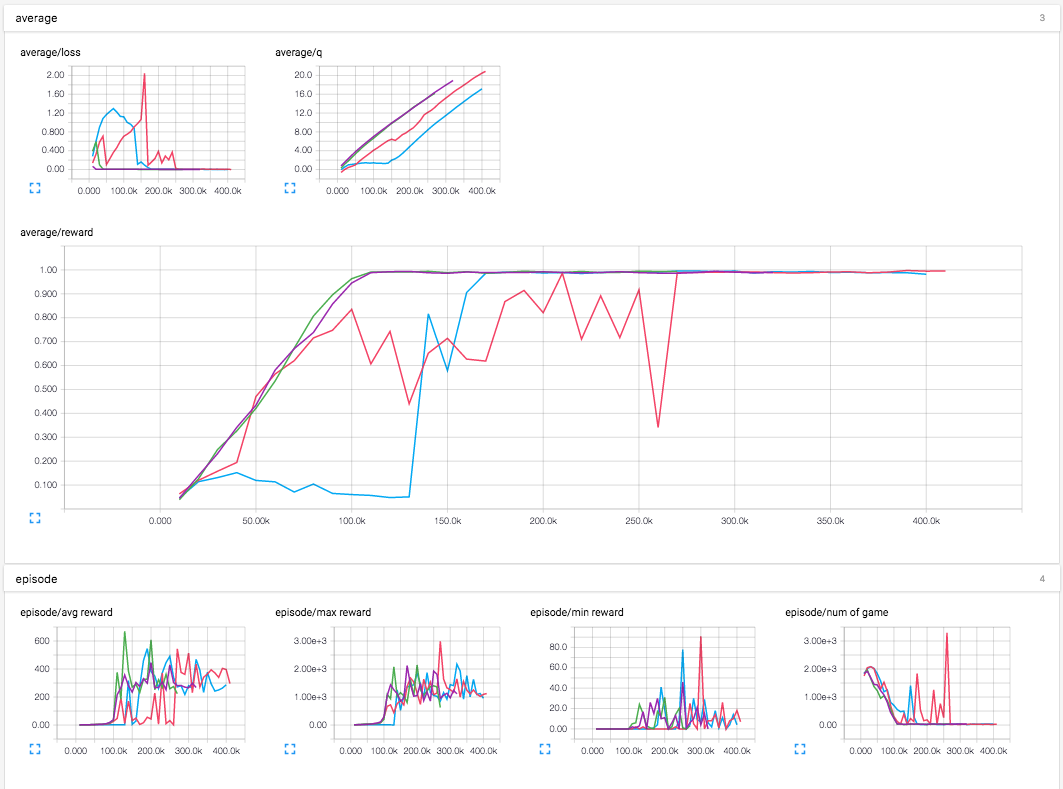
\includegraphics[width = \linewidth]{images/real_result}
    	\caption{The Result of Original Codes}
    	\label{fig::Result}
   \end{figure}
   
   In the above figure, DQN is purple line, DDQN is red and Dueling DDQN is blue, the green line is Dueling DQN, which I do not train.

\section{Conclusion}
In this report, I not only introduce and analyze some the basic theories and concepts of RL and DRL, but also show the test results of three DRL algorithms, DQN, Double DQN and Dueling network.

According to the test results of three models, I find that DQN model can have a palpale effect in a short training time. However, as the training proceeds, the effect will be decreasing, and the performance of DQN model is lack of stability. I think the primary cause is the DQN's overestimations, which can make it obtain rapid progress in the beginning but limit the pace and stability of training in the same time. 

On the contrary, the other two models do not perform well in the beginning. In the first 1 million episodes, they hardly get even one point, even if they get several points, these points all come from the same locations. After 3 millions episodes, they begin to perform better and make progress stably. Hence, I analyze that their training effect will have a gradual or even sudden rise when they have enough training, and their final performance will definitely be better than DQN model.

In this training section, I also met multiple difficulies in theories and practices. I got warm help from mentors and teammates, here I would like to extend my sincere thanks to them.

During this period of time, I do harvest a great deal. I have not only learned the knowledges I interested in, but also trained my own models.

Although the future learning would be harder, and time will less, I believe that I have prepared for the next training section and all coming difficulites.
{\small
\nocite{*}
\bibliographystyle{ieee}
\bibliography{reference}
}

\end{document}
